% !TeX root = ../correctness-deciders.tex

\newcommand{\HS}{Halting Segment\xspace}

\newpage
\section{Halting Segment}\label{sec:halting-segment}

\paragraph{Acknowledgement.} Sincere thanks to bbchallenge's contributor Iijil who initially presented this method and the first implementation\footnote{See: \url{https://discuss.bbchallenge.org/t/decider-halting-segment}.}. Other contributors have contributed to this method by producing alternative implementations (see Section~\ref{sec:hs-implem}) or discussing and writing the formal proof presented here: Mateusz Naściszewski (Mateon1), Nathan Fenner, Tony Guilfoyle, Justin Blanchard, Tristan Stérin (cosmo), and, Pavel Kropitz (uni).

\subsection{Overview}

\begin{figure}[h!]
  \centering
  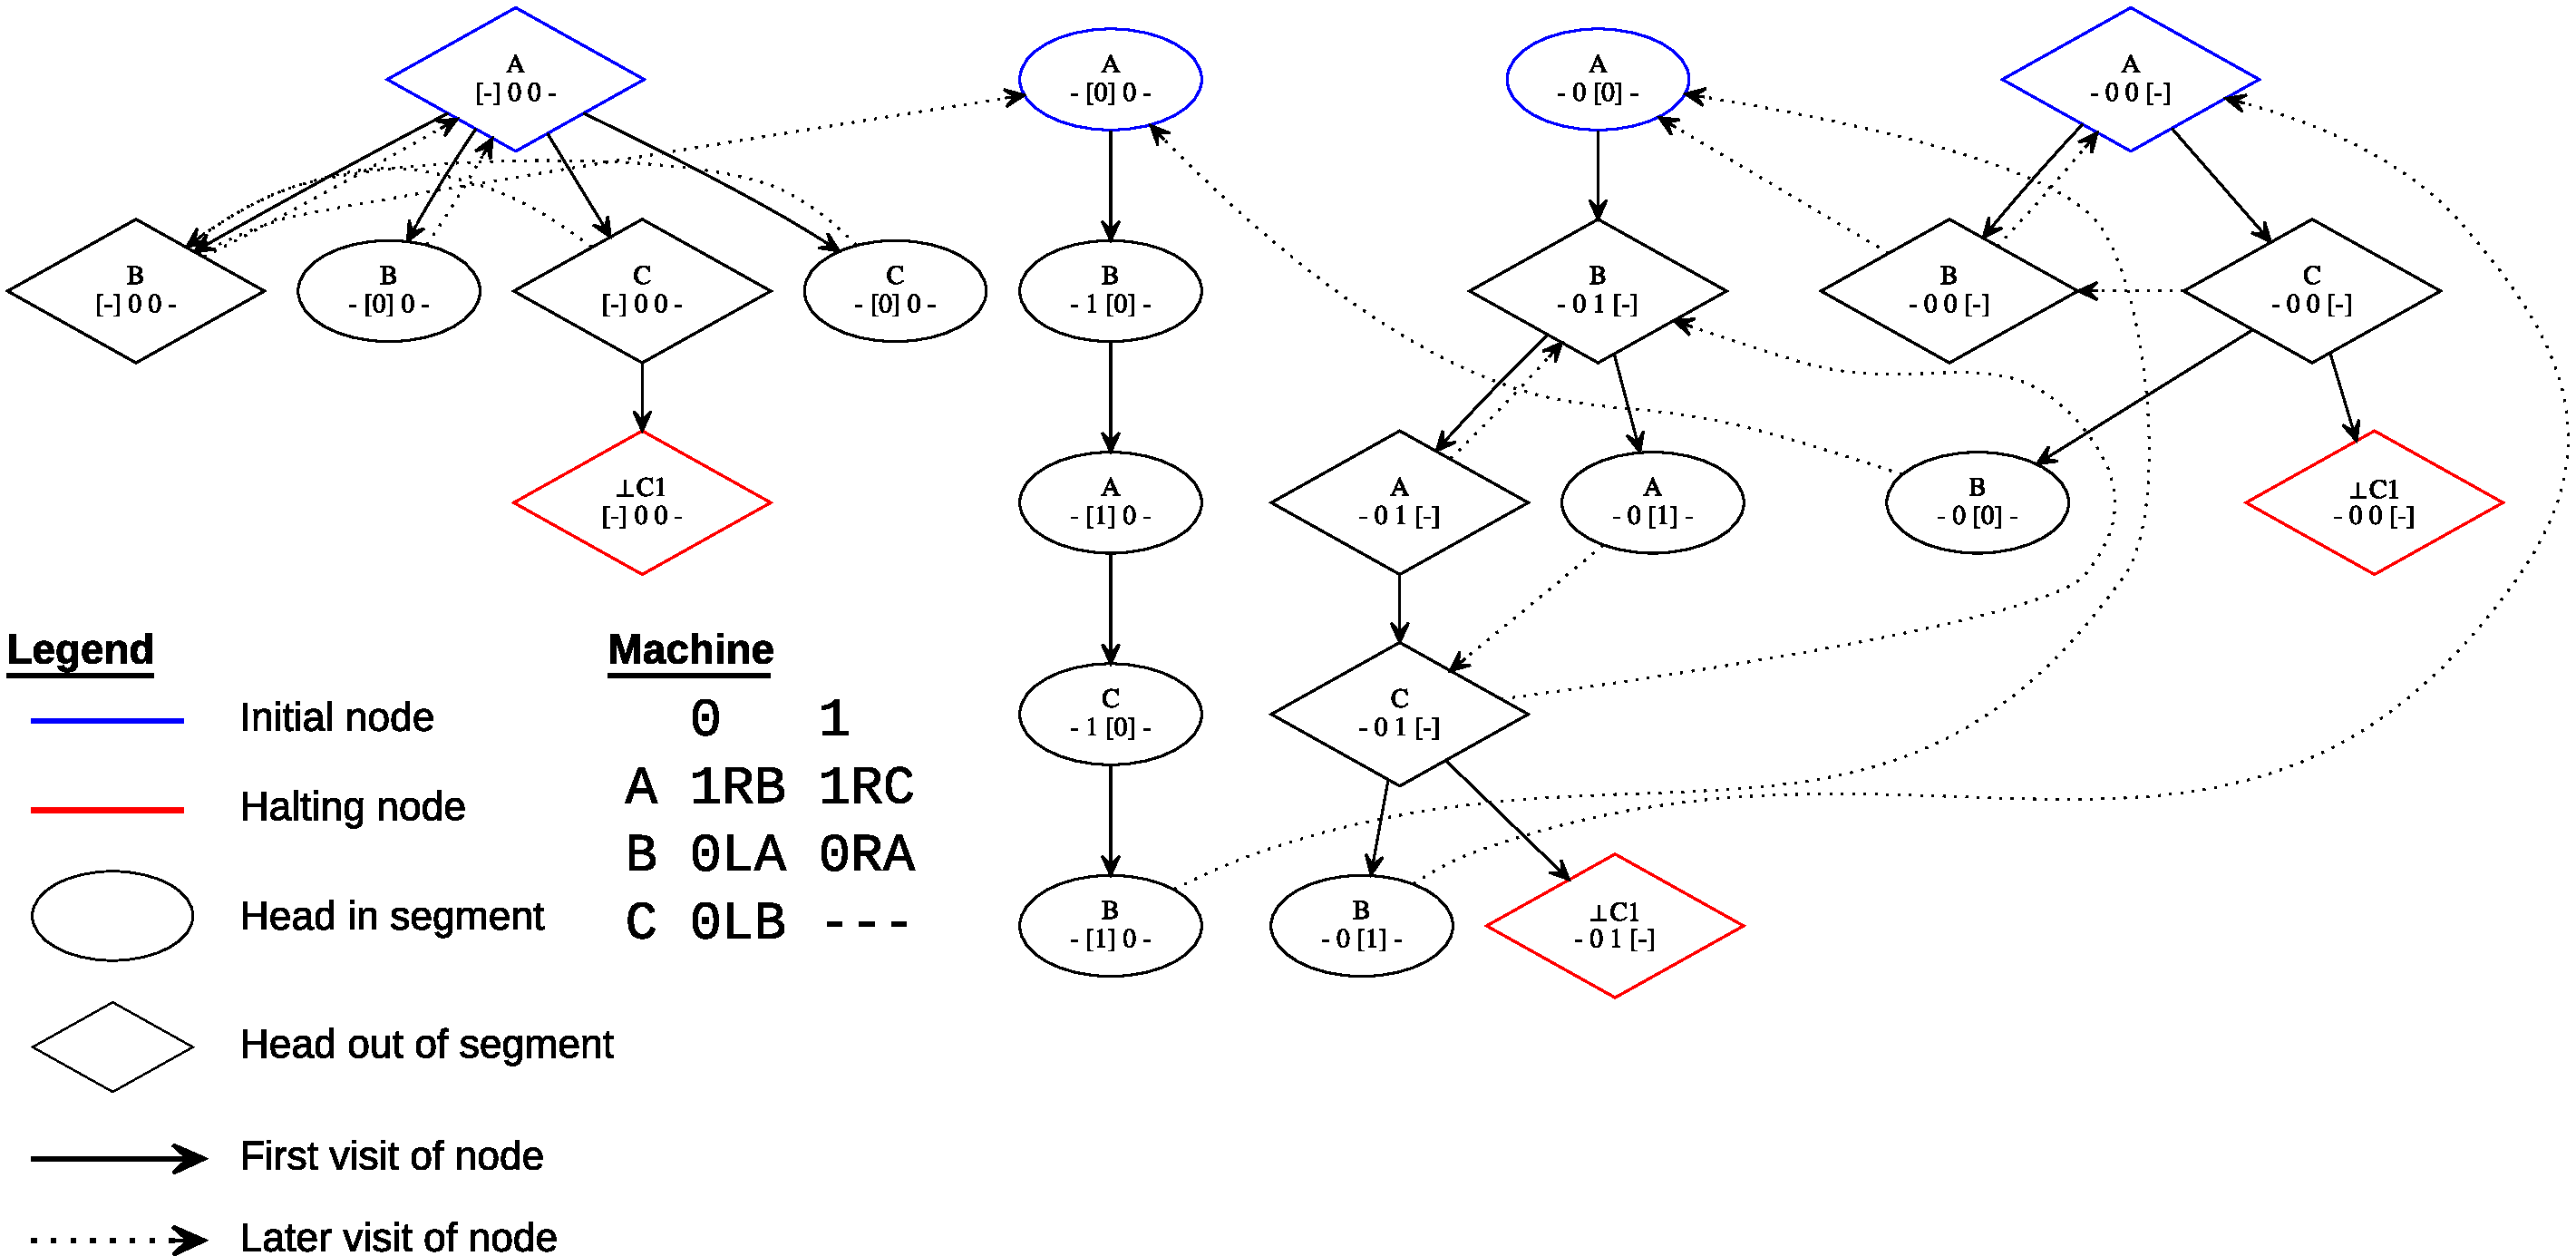
\includegraphics[width=1\textwidth]{figures/halting-segment/halting-segment.pdf}
  \caption{\HS graph for the 3-state machine \url{https://bbchallenge.org/1RB1RC_0LA0RA_0LB---} and segment size 2, see Definition~\ref{def:hs-graph}. Nodes of this graph correspond to \textit{segment configurations} (Definition~\ref{def:hs-conf}), i.e. configurations of the machine on a finite segment (here, of size 2). In a node, the machine's head position is represented between brackets and the symbol \texttt{-} represents the outside of the segment (either to the left or to the right). Nodes where the machine's head is within the segment (circle shape) only one have child corresponding to the next step of the machine and nodes where the head is outside of the segment (diamond shape) may have multiple children corresponding to all the theoretically possible ways (deduced from the machine's transition table) that the machine can enter the segment back or continue to stay out of it. In order to improve readibility, edges that revisit a node are dotted. The machine presented here does not halt because the halting nodes (red outline) that are reachable from the initial nodes (blue outline) do not cover all the positions of the segment (there is no halting node for any of the two internal positions of the segment), by contraposition of Theorem~\ref{th:hs}. }\label{fig:hs}
\end{figure}

The idea of the \HS technique is to simulate a Turing machine on a finite segment of tape. When the machine leaves the segment in a certain state, we consider all the possible ways that it can re-enter the segment or stay out of it, based on the machine's transition table. For a given machine and segment size, this method naturally gives rise to a graph, the \HS graph (formally defined in Definition~\ref{def:hs-graph}).

Figure~\ref{fig:hs} gives the \HS graph of the 3-state machine\footnote{We chose a 3-state machine in order to have a graph of reasonable size.} \url{https://bbchallenge.org/1RB1RC_0LA0RA_0LB---} for segment size 2. Let's describe this graph in more details:

\begin{itemize}
  \item Nodes correspond to \textit{segment configurations} (Definition~\ref{def:hs-conf}), i.e. the state in which the machine is together with the content of the segment and the position of the head in the segment (or outside of it). For instance, the leftmost node in blue and diamond shape in Figure~\ref{fig:hs} is \texttt{A [-] 0 0 -} which means that the machine is in state A, that the segment currently contains \texttt{0 0} and that the machine's head is currently outside of the segment, to the left of it.

  \item Initial nodes (blue outline) correspond to all sgement configurations that match the initial configuration of the machine (all-0 tape and state A), there are $n+2$ initial nodes with $n$ the size of the segment. Halting nodes (red outline) give the segment configurations where the machine has halted together with the halting transition that was used, for instance, in Figure~\ref{fig:hs}, the leftmost halting node \texttt{$\bot$ C1 [-] 0 0 -} signifies that the machine has halted ($\bot$), using halting transition \texttt{C1} (reading a 1 in state C), to the left of the segment which contains \texttt{0 0}.

  \item Nodes with a circle shape correspond to segment configurations where the tape's head is \textbf{inside} the segment. Such nodes only have one child, which corresponds to the next machine configuration.

  \item Nodes with a diamond shape correspond to segment configurations where the head is \textbf{outside} the segment, these nodes may have several children corresponding to all the ways that the head, in the current state, can stay outside of the segment or enter it back. For instance, the leftmost node in blue and diamond shape in Figure~\ref{fig:hs}, \texttt{A [-] 0 0 -}, has 4 children: \texttt{B [-] 0 0 -} and \texttt{B - [0] 0 -} and \texttt{C [-] 0 0 -} and \texttt{C - [0] 0 -}. This is because the transitions of the machine in state A are \texttt{1RB} and \texttt{1RC} and that the move \texttt{R} allows either to enter the segment back or to continue being out of it (if the head is far from the segment's left frontier). Note that the write symbol \texttt{1} of the transitions are ignored since we do not keep track of the tape outside of the segment.

  \item In order to increase the readability of Figure~\ref{fig:hs}, only one entrant edge for each node has been drawn with a solid line, corresponding to the first visit of that node in the particular order that the graph was visited. Later visits were drawn with a dotted line.
\end{itemize}

What is special about the \HS graph? We show in Theorem~\ref{th:hs} that if a machine halts, then, for all segment size, its \HS graph contains a set of halting nodes (red outline), for the same halting transition, that covers the entire segment and its outside, i.e. such that there is at least one such node per segment's position and outside of it (left and right). By contraposition, if there is no set of covering halting nodes for a halting transition, the machine does not halt. In Figure~\ref{fig:hs}, we deduce that machine \url{https://bbchallenge.org/1RB1RC_0LA0RA_0LB---} does not halt since the halting nodes of halting transition \texttt{C1} are \texttt{$\bot$ C1 [-] 0 0 -}, \texttt{$\bot$ C1 - 0 1 [-]} and \texttt{$\bot$ C1 - 0 0 [-]} which does not cover the entire segment (both internal segment postions are not covered).

Interestingly, \HS is the method that was used by Newcomb Greenleaf to prove\footnote{\url{http://turbotm.de/~heiner/BB/TM4-proof.txt}} that Marxen \& Buntrock's chaotic machine\footnote{\url{https://bbchallenge.org/76708232}} \cite{Marxen_1998} does not halt.

\subsection{Formal proof}

\begin{definition}[Segment configurations]\label{def:hs-conf}
  Let $n \in \N = \{0, 1, 2 \dots\}$ a natural number called \textit{segment size}. A \textit{segment configuration} is a 3-tuple: (i) state, (ii) $w \in \{0,1\}^n$ which is the segment's content and (iii) the position of the machine's head is an integer $p \in \llbracket -1, n \rrbracket$ where positions $\llbracket 0,n \llbracket$ correspond to the interior of the segment, position $-1$ for outside to the left and $n$ for outside to the right. \textit{Halting segment configurations} are segment configurations where the state is $\bot$ and with an additional information (iv) of which halting transition of the machine has been used to halt.
\end{definition}

\begin{example}
  In Figure~\ref{fig:hs} we have $n=2$ and, the leftmost node in blue and diamond shape corresponds to segment configuration \texttt{A [-] 0 0 -} (i) state A, (ii) $w = \texttt{00}$ and (iii) $p = -1$. The rightmost node in red and diamond shape corresponds to halting segment configuration $\bot$ \texttt{C1 - 0 0 [-]} (i) state $\bot$, (ii) $w = \texttt{00}$, (iii) $p = 2$ and (iv) halting transition \texttt{C1}.
\end{example}

\begin{definition}[\HS graph]\label{def:hs-graph}
  Let $\mathcal{M}$ be a Turing machine and $n \in \N$ a segment size. The \HS graph for $M$ and $n$ is a directed graph where the nodes are segment configurations (Definition~\ref{def:hs-conf}). The graph is generated from $n+2$ \textit{initial nodes} (blue outline in Figure~\ref{fig:hs}) that are all in state A with segment content $0^n$ ($n$ consecutive 0s) but where the head is at each of the $n+2$ possible positions, one per each initial node, see the blue nodes in Figure~\ref{fig:hs} for an example.
  Then, edges that go out of a given node $r$ are defined as follows:
  \begin{itemize}
    \item If $r$'s head position is inside the segment (circle nodes in Figure~\ref{fig:hs}), then $r$ only has one child corresponding to the next simulation step for machine $\mathcal{M}$. For instance, in Figure~\ref{fig:hs}, node \texttt{A - [0] 0 -} has a unique child \texttt{B - 1 [0] -}, following machine's transition \texttt{A0} which is \texttt{1RB}. That child can be a halting segment configuration if the transition to take is halting.
    \item If $r$'s head position is outside the segment (diamond nodes in Figure~\ref{fig:hs}), then, we consider each transition of $r$'s state. There are three cases:
          \begin{enumerate}
            \item If the transition is halting, we add a child to $r$ which is the halting segment configuration node corresponding to this transition. For instance, in Figure~\ref{fig:hs}, \texttt{C [-] 0 0 -} has halting child $\bot$ \texttt{C1 [-] 0 0 -} corresponding to halting transition \texttt{C1}.
            \item If the transition's movement goes further away from the segment (e.g. we are to the left of the segment, $p=-1$, and the transition movement is \texttt{L}), we add one child for this transition that only differs from its parent in the new state that it moves into. For instance, in Figure~\ref{fig:hs}, \texttt{A - 0 0 [-]} has child $\bot$ \texttt{B - 0 0 [-]} for transition \texttt{A0} which is \texttt{1RB}.
            \item If the transition's movement goes in the direction of the segment (e.g. we are to the left of the segment, $p=-1$, and the transition movement is \texttt{R}), we add two children for this transition. One corresponding to the case where that movement is made at the border of the segment and allows to re-enter the segment and the other one corresponding to the case where that movement is made farther away from the border and does not re-enters yet. For instance, in Figure~\ref{fig:hs}, node \texttt{A [-] 0 0 -} has children \texttt{B [-] 0 0 -} and \texttt{B - [0] 0 -} for transition \texttt{A0} which is \texttt{1RB}.
          \end{enumerate}
  \end{itemize}

  Halting nodes are nodes corresponding to halting segment configurations (red outline in Figure~\ref{fig:hs}).

\end{definition}

\begin{theorem}[\HS]\label{th:hs}
  Let $\mathcal{M}$ be a Turing machine and $n \in \N$ a segment size. Let $G$ be the \HS graph for $\mathcal{M}$ and $n$ (Definition~\ref{def:hs-graph}). If $\mathcal{M}$ halts in halting transition $T$ when started from state A and all-0 tape, then $G$ must contain a halting node for transition $T$ for each of the $n+2$ possible values of the head's position $p \in \llbracket -1, n \rrbracket$.
\end{theorem}
\begin{proof}
  Consider the trace of configurations of $\mathcal{M}$ (full configurations, not segment configurations, as defined in Section~\ref{sec:cyclers}) from the initial configuration (state A and all-0 tape) to the halting configuration which happens using halting transition $T$. Starting from the halting configuration, construct the halting segment configuration (with segment size $n$) for $T$ using any position $p \in \llbracket -1, n \rrbracket$ in the segment and fill the segment's content from what is written on the tape around the head in the halting configuration of $\mathcal{M}$. From there, work your way up to the initial configuration: at each step construct the associated segment configuration. This sequence of segment configurations constitute a set of nodes in the \HS graph $G$ of $\mathcal{M}$ for segment size $n$ such that each node points to the next one. At the top of that chain there will be a node matching the initial configuration: state A, all-0 segment and head position somewhere in $\llbracket -1, n \rrbracket$, i.e. an initial node.

  Hence we have shown that all halting nodes for transition $T$ for each of the $n+2$ possible values of the head's position $p \in \llbracket -1, n \rrbracket$ are reachable from some initial node(s).
\end{proof}

\begin{remark}
  By contraposition of Theorem~\ref{th:hs}, if, for all halting transitions $T$ there is at least one halting node (red outline in Figure~\ref{fig:hs}) for some position in the segment that is not reachable from one of the initial node (blue outline in Figure~\ref{fig:hs}) then the machine does not halt. That way, in Figure~\ref{fig:hs}, we can conclude that machine\url{https://bbchallenge.org/1RB1RC_0LA0RA_0LB---} does not halt since the halting nodes of halting transition \texttt{C1} are \texttt{$\bot$ C1 [-] 0 0 -}, \texttt{$\bot$ C1 - 0 1 [-]} and \texttt{$\bot$ C1 - 0 0 [-]} which does not cover the entire segment (both internal segment postions are not covered).

  Note that if all of the segment's positions are covered for some halting transition, we cannot conclude that the machine does not halt, but it does not mean that the machine necessarily halts either.
\end{remark}

\begin{remark}
  Some non-halting machines cannot be decided using \HS for any segment size. Such a machine is for instance \url{https://bbchallenge.org/1RB---_1LC0RB_1LB1LA}.
\end{remark}

\subsection{Implementations and results}\label{sec:hs-implem}


Here are the implementations of the method that were realised, almost all of them construct the \HS graph from the halting nodes (backward implementation) instead than from the initial nodes (forward implementation):

\begin{enumerate}
  \item Iijil's who originally proposed the method, \url{https://github.com/bbchallenge/bbchallenge-deciders/tree/main/decider-halting-segment}, and was independently reproduced by Tristan Stérin (cosmo) \url{https://github.com/bbchallenge/bbchallenge-deciders/tree/main/decider-halting-segment-reproduction} (backward implementation)
  \item Mateusz Naściszewski (Mateon1)'s: \url{https://gist.github.com/mateon1/7f5e10169abbb50d1537165c6e71733b} (forward implementation)
  \item Nathan Fenner's which has the interesting feature of being written in a language for formal verification (Dafny): \url{https://github.com/Nathan-Fenner/bbchallenge-dafny-deciders/blob/main/halting-segment.dfy} (backward implementation)
  \item Tony Guilfoyle: \url{https://github.com/TonyGuil/bbchallenge/tree/main/HaltingSegments} (backward implementation)
\end{enumerate}

We will be only discussing the details and results of Iijil's implementation (1) as it was the first implementation to be proposed and that it also was reproduced independently with exactly matching results.

This implementation is a bit different from what is presented in this document because the \HS graph is constructed backward (i.e. from the halting nodes instead than from the initial nodes). Also, the method adopts a lazy strategy consisting in testing only odd segment sizes (up to size $n_\text{max}$) and placing the head's position at the center of the tape. Finally, the information of state is not stored for nodes where the head is outside the segment. These implementation choices make the implementation a bit weaker than what was presented here.

Nonetheless, results are impressive, for $n_\texttt{max} = 13$, the method decides 1,002,808 machines out of the 1,538,624 remaining after backward reasoning (see Section~\ref{sec:backward-reasoning-results}). Hence, after \HS, we have 535,816 machines left to be decided\footnote{In fact 535,801 because 15 additional translated cyclers were decided, including some Skelet's machines.}.
